\documentclass{beamer}

\usepackage{fontspec,xunicode,xltxtra}
\usepackage[english]{babel}
\usepackage{microtype}
\usepackage{default}	

\usepackage[]{hyperref}
\hypersetup{
	colorlinks=true}
\usetheme{simple}
\usepackage{graphicx}
\usepackage[justification=centering]{caption}
\usepackage{subcaption}
\usepackage{listings}
\usepackage{pstricks}
\setmainfont{Fira Sans}
\setsansfont{Noto Sans}
\setmonofont{Fira Mono}
\captionsetup[subfigure]{labelformat=empty}
\captionsetup[figure]{labelformat=empty}
\setbeamertemplate{caption}{\raggedright\insertcaption\par}
\setbeamerfont{frametitle}{size=\LARGE}
\newfontfamily\DejaSans{DejaVu Sans}
\setbeamerfont{title}{family=\texttt,size=\huge}
\usepackage[scale=2]{ccicons}
\newfontfamily\unicodefun[Ligatures=TeX]{Symbola}
\newfontfamily\unicodefun{Droid Sans}
\title{Graphical Temporal Structured Programming}
\subtitle{}
\date{}
\author{Jean-Michaël Celerier$\mathsf{^{1,2,3}}$~\\ Myriam Desainte-Catherine$\mathsf{^{2,3}}$~\\ Jean-Michel Couturier$\mathsf{^{1}}$}
\institute{1: Blue Yeti~\\2: LaBRI~\\3: PoSET}
\usepackage{tikz}

\newsavebox{\codebox}% For storing listings
\begin{document}
    
\maketitle
\begin{frame}
	\tableofcontents
\end{frame}
\section{Introduction}

\begin{frame}
    \frametitle{Position}    
    \Large
    % TODO diagramme interactivité de la pres 1A
    Authoring interactivity ?
    When A then B : programming.
    
    Code-first environments.
    
\end{frame}

\begin{frame}
    \frametitle{Inspiration}
    \Large
    John Cage's Two, Klavierstücke XI
\end{frame}

\section{Description}
\begin{frame}
    \Huge
    \centering{Vocabulary}
\end{frame}    
\begin{frame}[plain]
    \begin{tikzpicture}[remember picture,overlay]
    \node[at=(current page.center)] {
        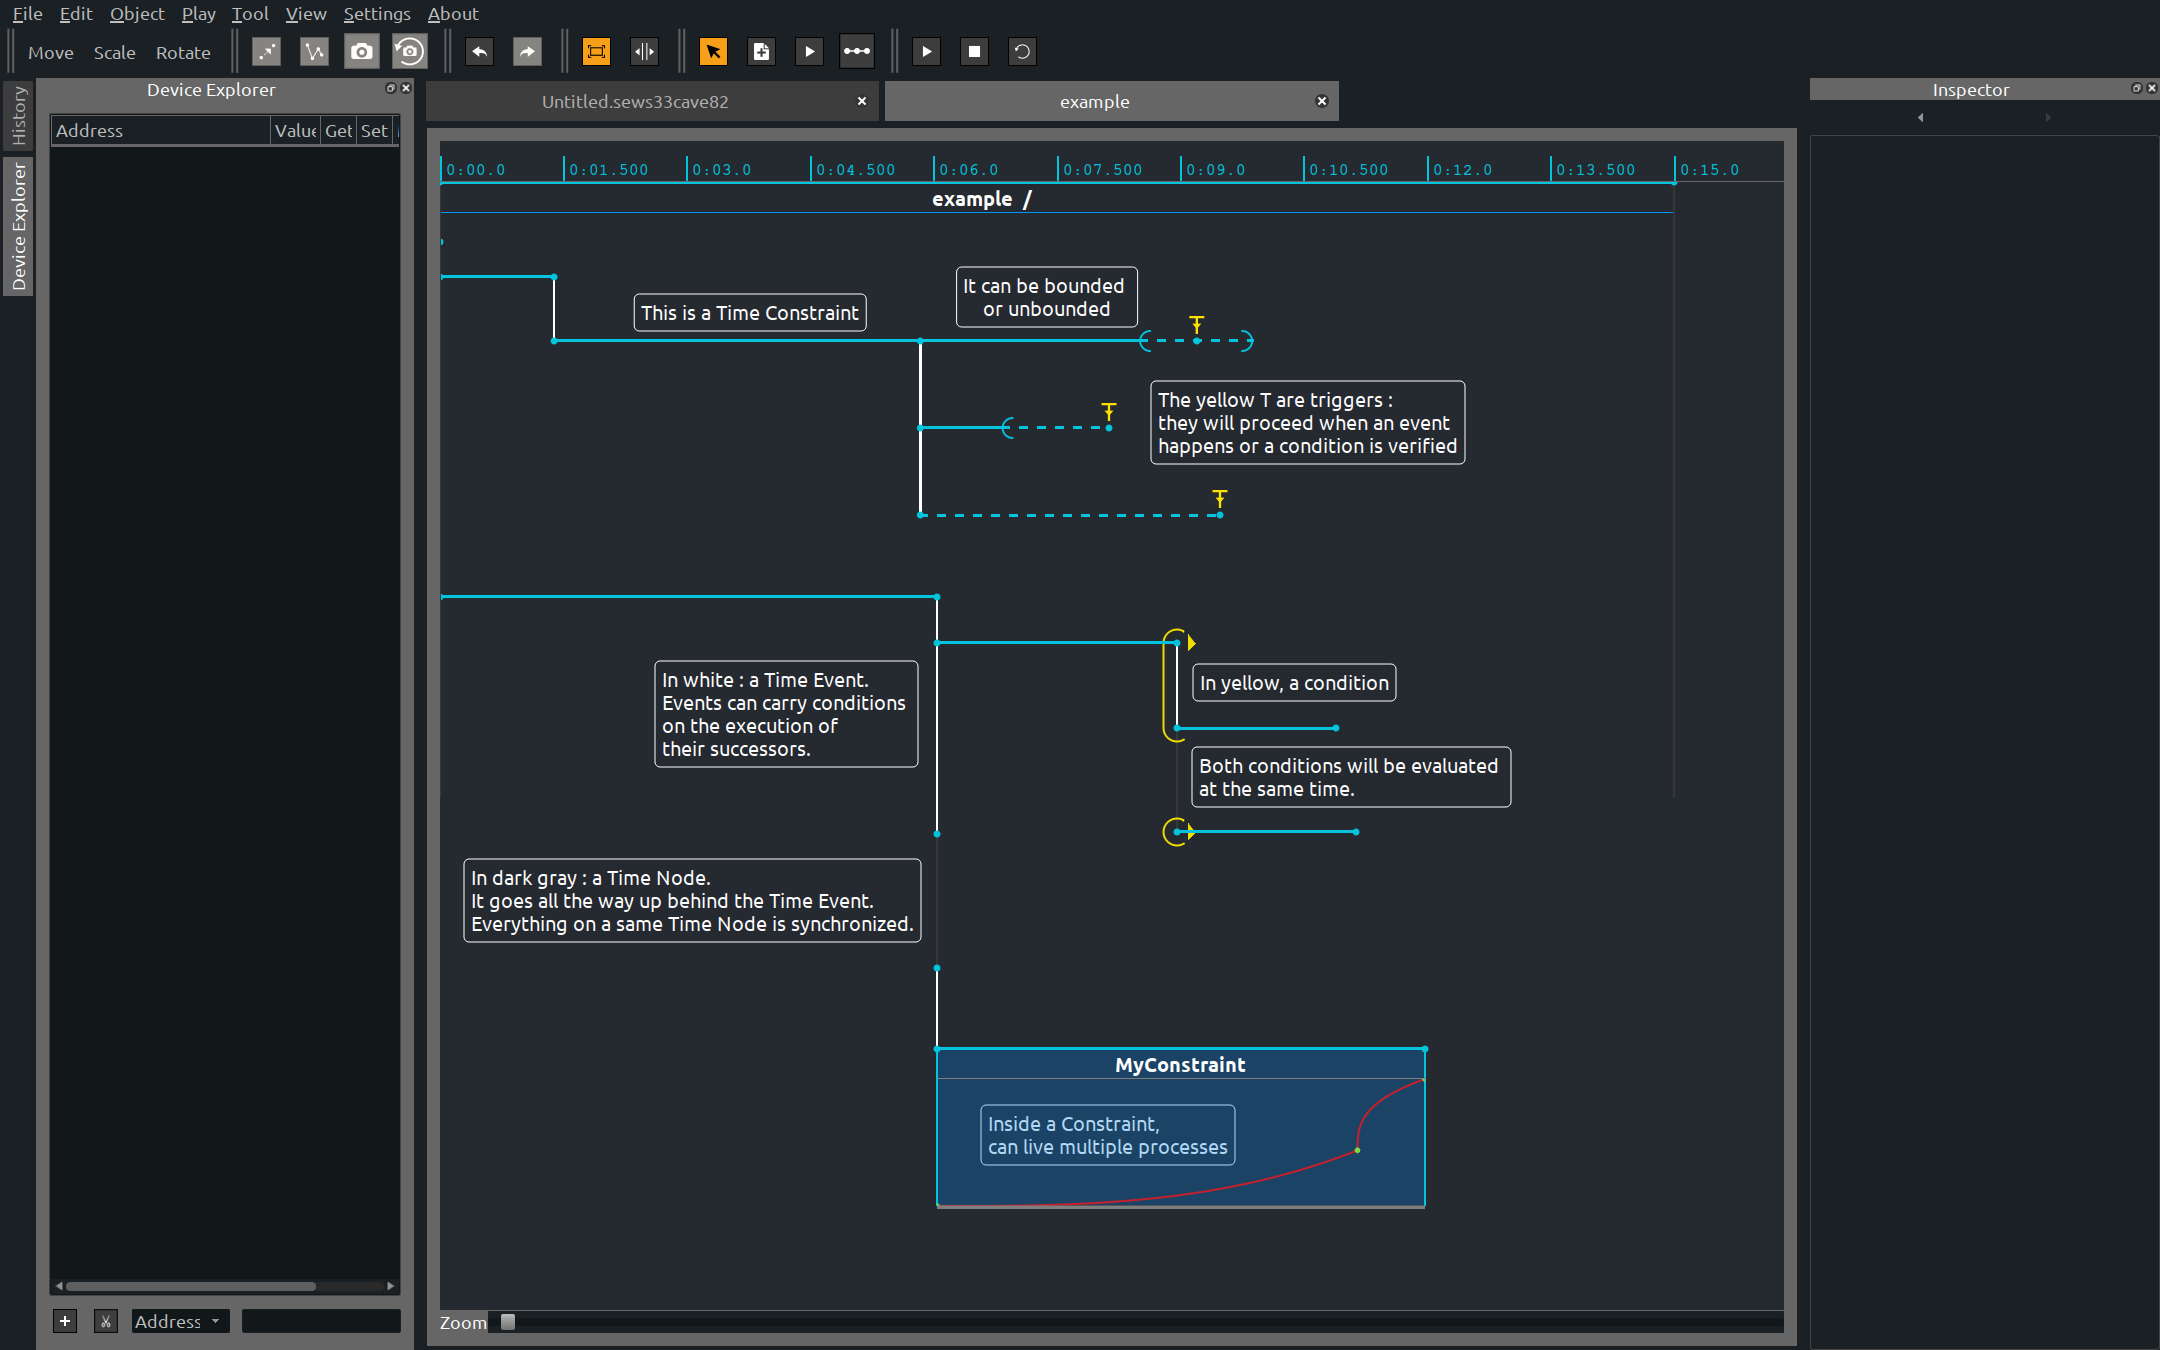
\includegraphics[width=1.5\paperwidth]{images/example.png}
     };
     \end{tikzpicture}
\end{frame}

\begin{frame}
    Playhead semantics
\end{frame}

\begin{frame}
    \Large
    \frametitle{Loops}  
\end{frame}

\begin{frame}
    \Large
    \frametitle{Data tree}  
\end{frame}

\begin{frame}
    \Large
    \frametitle{Code}  
\end{frame}

\section{Authoring}
\begin{frame}
    \frametitle{"Procedural"}
\end{frame}
\begin{frame}
    \frametitle{"Event-driven"}
\end{frame}


\subsection{Audio processes}
\begin{frame}	
    \frametitle{Audio processes}    
    \LARGE
    \begin{itemize}
        \item Soundfile reading.
        \item Real-time input.
        \item Effect chains (Faust, LV2 in-progress).
        \item Audiograph features~\\$\rightarrow$ send and return from different points in the score.
        \item Mixing.
    \end{itemize}    
\end{frame}

\section{Method}
\begin{frame}
    \frametitle{The i-score audio graph}    
\end{frame}


\section{Demo}

\begin{frame}
    \Huge
    \centering{Demo}~\\\vspace{1cm}
    \url{icmc.blueyeti.fr}
\end{frame}

\begin{frame}
	\frametitle{Future} 
	\Large
	\begin{itemize}
		\item<1> Integrated input recording.
		\item<2> Real-time audio input delaying and reuse.
		\item<3> Deep MIDI integration, piano roll, etc.
		\item<4> Hierarchic temporal signatures.
        \item<5> Spatialisation ?
		
	\end{itemize}
\end{frame}    


\begin{frame}[allowframebreaks]%in case more than 1 slide needed
    
    %remove the icon
    \setbeamertemplate{bibliography item}{}
    
    %remove line breaks
    \setbeamertemplate{bibliography entry title}{}
    \setbeamertemplate{bibliography entry location}{}
    \setbeamertemplate{bibliography entry note}{}
    
    {\footnotesize
        \nocite{*}
        \bibliographystyle{IEEEtran}
        \bibliography{icmc2016}
    }
\end{frame}

\begin{frame}
    \frametitle{Links} 
    \Large
    \begin{itemize}
        \setlength\itemsep{1em}
        \item \textbf{i-score} : \url{www.i-score.org}
    \end{itemize}
        
    \centering
    \vspace{2em}
    \Large{Thanks ! Questions ?}
    \vspace{2em}
    
    \tiny{Uses the Beamer 'simple' theme, Facundo Muñoz; and Mozilla's Fira font family}
\end{frame}
\end{document}
